%% -*- coding: utf-8 -*-
\documentclass[12pt,pagesize,paper=landscape,paper=192mm:108mm]{scrbook}
% 1920x1080 1280x720
\areaset[current]{192mm}{108mm}
\usepackage[T2A]{fontenc}
\usepackage[utf8]{inputenc}
\usepackage[english,russian]{babel}
\usepackage{microtype}
\usepackage{misccorr}
\usepackage{cmap}
%\usepackage[unicode=true]{hyperref}
\usepackage{graphicx}
\usepackage{amssymb}
\usepackage{amsmath}
%\usepackage{srcltx}
\usepackage{textcomp}
\usepackage{xspace}
%научные символы и смайлики \smiley \frownie
\usepackage{wasysym}
\usepackage{ccicons}
\usepackage{url}
\DeclareMathOperator{\Tr}{Tr}
%перенос формул в тексте
\newcommand*{\hm}[1]{#1\nobreak\discretionary{}%
  {\hbox{$\mathsurround=0pt #1$}}{}}
\renewcommand{\epsilon}{\varepsilon}

\begin{document}
\begin{titlepage}
  \vspace*{-0.5em}
  \begin{center}    
    \hspace*{3em}
    \begin{minipage}[t]{3em}
      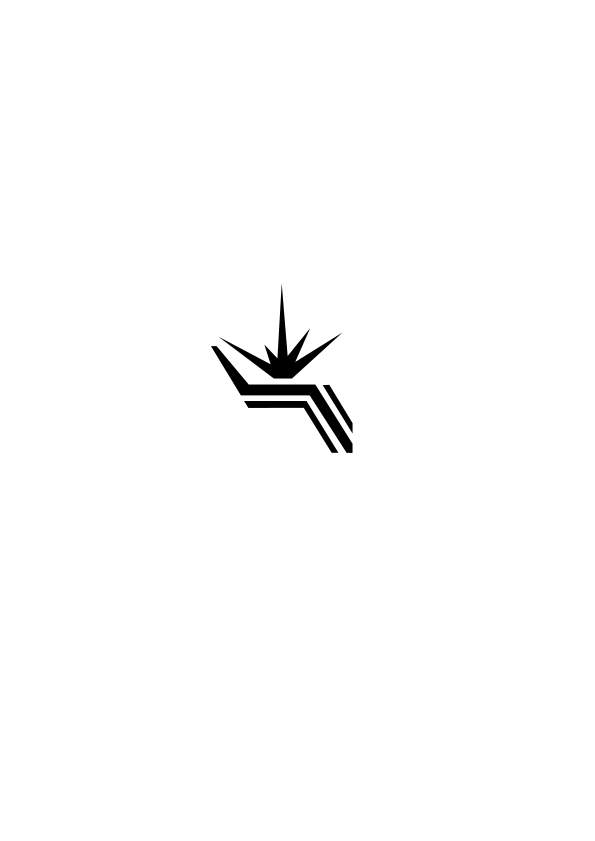
\includegraphics[width=\textwidth]{../BINP-logo}
    \end{minipage}\hfill
    \begin{minipage}{0.23\linewidth}
    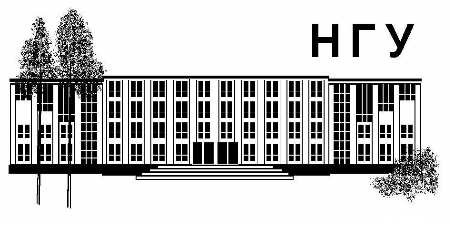
\includegraphics[width=\textwidth]{../NSU-logo}
    \end{minipage}
    \hfill
    \hspace*{6em}

    Кафедра физики элементарных частиц физического факультета НГУ
    \smallskip

    \Large
    Профессор Андрей Грабовский
    
    \smallskip

    \huge
    \textbf{Квантовая хромодинамика}
    \smallskip

    \Large
    Лекция № 24
    \vfill

    \normalsize
    \begin{minipage}{0.9\linewidth}
      Вклад резонанса и состояний континуума в поляризационный
      оператор фотона. Дисперсионное соотношение, дисперсионное
      соотношение с вычитанием. Правила сумм для
      моментов. Преобразование Бореля для поляризационного оператора и
      правила сумм. Вакуумные конденсаты. Операторное разложение.
      Операторное разложение для Т"=произведения электромагнитных токов
      "--- поляризационного оператора. Размерности коэффициентных функций
      и матричных элементов локальных операторов.
    \end{minipage}
    \vfill

    \normalsize \ccbysa\hspace{0.5em}  Новосибирск 2024
  \end{center}
\end{titlepage}
\end{document}

%%% Local Variables:
%%% mode: latex
%%% TeX-master: t
%%% End:
